\documentclass{beamer}
\usepackage[spanish]{babel}
\selectlanguage{spanish}
\usepackage{graphicx}
\usepackage{float}
\usepackage{graphicx,subcaption}
\usepackage[utf8]{inputenc}
\usepackage[font=scriptsize,labelfont=bf]{caption}
\usepackage{ragged2e}
\usepackage{booktabs}
\usepackage{tikz}
\usepackage{listings}

\graphicspath{{/home/daniu/Documentos/charla_GIS/figuras/}}

\usetheme{Madrid}

\title[Python para SIG]{Caracterización espacio-temporal de la clorofila en el mar argentino mediante herramientas de Python}
\subtitle{}
\author[Risaro, Daniela B]{Daniela B. Risaro\inst{1} \inst{2}}

\institute[SHN-UBA] % (optional)
{
	\inst{1}%
	Departamento de Oceanografía\\
	Servicio de Hidrografía Naval (SHN)
	\and
	\inst{2}%
	Facultad de Cs Exactas y Naturales\\
	Universidad de Buenos Aires (UBA)
}
\date{\today}

\begin{document}
\begin{frame}
 \titlepage
\end{frame}

\begin{frame}
\frametitle{Esquema }
\tableofcontents
\end{frame} 

\section{Motivación}

\begin{frame}
 \frametitle{El mar argentino}
 caracteristicas del mar argentino y el area de estudio
 
 Caracterizar la variabilidad temporal y espacial de la clorofila en el mar argentino
 
\begin{figure}
 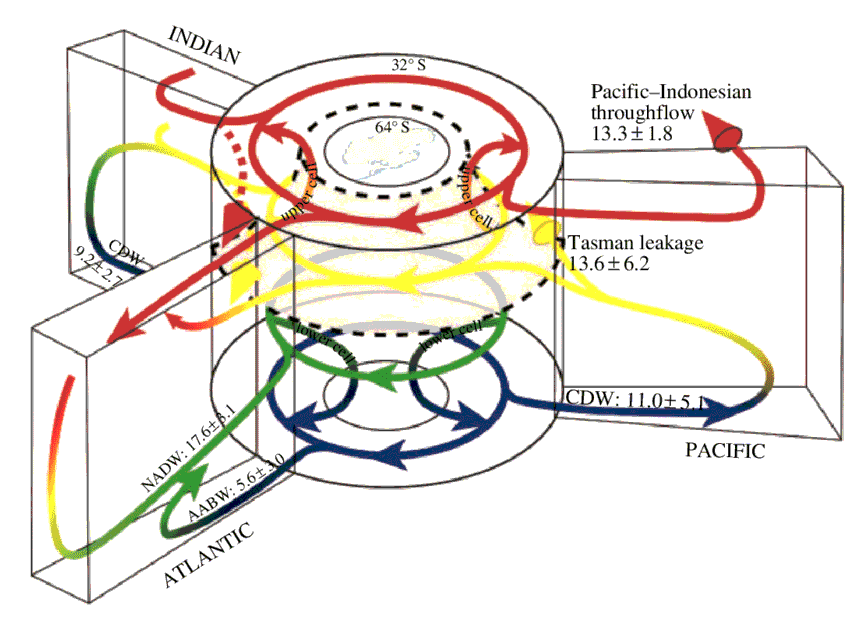
\includegraphics[scale=0.4]{moc.png}
\caption{Mapa del area de estudio y algo sobre cloro a}
 \end{figure}
\end{frame}


\section{Datos de clorofila}

\begin{frame}[t]
 \frametitle{Datos disponibles - clorofila-a}
 

  \begin{itemize}
   \item<1-> Mediciones in-situ \pause $\rightarrow$ muy escasas
   \item<3-> Satelitales 
      


 
   \begin{figure}
   	
   	\begin{tikzpicture}
   	\node[anchor=south west,inner sep=0] at (0,0) {\includegraphics<4->[scale=0.9]{global_ocean_color_sensors.pdf}};
   	\draw<5->[red,thick,rounded corners] (3.55,2.1) rectangle (5.8,2.45);
   	\draw<6->[red,thick,rounded corners] (4.3 ,2.55) rectangle (7.7, 2.9);
   	\end{tikzpicture}	
   \end{figure}

\item[]<7->\tiny{Fuente: \href{https://oceancolor.gsfc.nasa.gov/docs/odps_opdsmp.may2018.pdf}{\beamergotobutton{Link}}}
  \end{itemize}
\end{frame}


\begin{frame}[t]
\frametitle{Archivos}

\begin{itemize}
	\item<1->[] ¿Dónde encuentro esta información? $\rightarrow$ Ocean color \href{https://oceancolor.gsfc.nasa.gov/}{\beamergotobutton{Link}}

	\item<2->[] Niveles de procesamiento:
\begin{itemize}
	\item L1 y L2
	\item L3 $\rightarrow$ grillados 
\end{itemize}

   \begin{figure}
	
	\begin{tikzpicture}
	\node[anchor=south west,inner sep=0] at (0,0) {\includegraphics<4->[scale=0.22]{L3browser.png}};
	\draw<5->[red,thick,rounded corners] (1.5, 2.7) rectangle (2.5, 2.9);
	\draw<6->[red,thick,rounded corners] (3.7, 2.7) rectangle (4.5, 2.9);
	\draw<7->[red,thick,rounded corners] (6.2, 2.7) rectangle (7, 2.9);
	\draw<8->[red,thick,rounded corners] (8.5, 2.7) rectangle (9.5, 2.9);
	\draw<9->[red,thick,rounded corners] (0.15, 2.3) rectangle (6, 2.5);
	\draw<10->[black,thick,rounded corners] (7.3, 3) rectangle (9.1, 3.4);			
	\end{tikzpicture}	
	
   \end{figure}

\end{itemize}
\end{frame}


\begin{frame}[fragile]
\frametitle{Archivos}

Luego de seleccionar la opcion 'Mapped' uno obtiene una lista de links de archivos netCDF (.nc)
\\~\\
\url{https://oceandata.sci.gsfc.nasa.gov/cgi/getfile/A20022132002243.L3m_MO_CHL.x_chlor_a.nc} \href{https://oceandata.sci.gsfc.nasa.gov/cgi/getfile/A20022132002243.L3m_MO_CHL.x_chlor_a.nc}{\beamergotobutton{Link}}
\\~\\

\pause
Si son varios archivos:
\begin{itemize}
	\item generar un archivo datos.txt 
	\item ejecutar en la terminal el comando 
	
	\begin{lstlisting}[language=bash, basicstyle=\scriptsize]
	cd /home/daniu/Documentos/charla_gis/
	wget -i datos.txt  
	\end{lstlisting}
\end{itemize}

\end{frame}


\begin{frame}[fragile]
\frametitle{Archivos}

Un archivo netCDF (Network Common Data Form) es un formato que guarda datos multidimensionales para variables climáticas, por ejemplo:

\begin{itemize}
	
	\item TSM (tiempo, latitud, longitud)
	\item Taire (tiempo, latitud, longitud, presion)
	\item clorofila-a (tiempo, latitud, longitud)
	
\end{itemize}

\pause

El archivo .nc tiene un \textit{header} que contiene toda la información sobre las dimensiones y atributos de las variables, pero no los valores en si. Los datos, están comprimidos en la \textit{data-part} del archivo. 

\end{frame}


\begin{frame}[fragile]
\frametitle{Archivos}

Para visualizar la información del \textit{header} podemos ejecutar en la terminal:

\begin{lstlisting}[language=bash, basicstyle=\scriptsize]
cd /home/daniu/charla_gis/
ncdump -h A20022132002243.L3m_MO_CHL.x_chlor_a.nc
\end{lstlisting}

y obtenemos lo siguiente:

\begin{figure}

\begin{tikzpicture}
   \node[anchor=south west,inner sep=0] at (0,0) {\includegraphics<1->[scale=0.2]{ncdump-console.png}};
   \draw<3->[->] (-0.9, 5.3) -- (-0.3, 5.3);
   \draw<4->[->] (-0.9, 4.7) -- (-0.3, 4.7);
   \draw<5->[->] (-0.9, 1.2) -- (-0.3, 1.2);      
\end{tikzpicture}

\end{figure}

\end{frame}

\section{Python workflow}

\begin{frame}[fragile]
\frametitle{Manipulación .nc en python}

En Python hay una libreria especializada en la manipulación de archivos netCDF \texttt{xarray} llamada (más info en: \href{http://xarray.pydata.org/en/stable/}{\beamergotobutton{Link}})

\begin{lstlisting}[language=python, basicstyle=\scriptsize]

import xarray as xr

dire = '/home/daniu/Documentos/charla_gis/'
filename = 'A20021822019212.L3m_MC_CHL_chlor_a_9km.nc'
data = xr.open_dataset(dire + filename)

\end{lstlisting}

\begin{figure}
	
	\begin{tikzpicture}
	\node[anchor=south west,inner sep=0] at (0,0) {\includegraphics<1->[scale=0.15]{dataset-diagram.png}};
	\draw<3->[black,thick,rounded corners] (1.3,2.2) circle (0.35cm);
	\draw<3->[black,thick,rounded corners] (4.7,2.2) circle (0.35cm);
	\end{tikzpicture}
	
\end{figure}
\end{frame}


\begin{frame}[fragile]
\frametitle{Operaciones con xarray}

\begin{lstlisting}[language=python, basicstyle=\scriptsize]
import xarray as xr

dire = '/home/daniu/Documentos/charla_gis/'
filename = 'A20022132002243.L3m_MO_CHL.x_chlor_a.nc'
data_chl = xr.open_dataset(dire + filename)

print(data)

chl_a = data_chl.sel(slice(), slice())

\end{lstlisting}

\end{frame}


\begin{frame}[fragile]
\frametitle{Mapas}

\end{frame}

\begin{frame}[fragile]
\frametitle{Series temporales}

\end{frame}

\section{Resultados del mar Argentino}
\begin{frame}
\frametitle{Construccion series temporales}

\begin{itemize}
	\item Se realizo una serie que unifica a SWFs y MODIS en cada punto de grilla segun la metodología de \cite{marrari}
\end{itemize}

\end{frame}


%
%
%\section{Conclusiones}
%\begin{frame}
%\frametitle{Conclusiones}
%\vspace{-0.3cm}
% \begin{itemize}
%  \item<1-> Los autores realizan un estudio de los modos de variabilidad de anomalías de SST en los océanos australes a partir de un ensamble de modelos del CMIP5.
%  \item<2->  Los tres modos principales son:
%        \begin{itemize}
%         \item EOF-1: Modo anular
%         \item EOF-2: Patrón monopolar con máximos en el Atlántico Sur
%         \item EOF-3: Dipolo del Pacífico Sur
%        \end{itemize}
%  \item<3->  Los períodos de oscilación de cada modo:
%        \begin{itemize}
%         \item EOF-1: Modo anular $\Rightarrow$ interanuales a decadales
%         \item EOF-2: Patrón monopolar con máximos en el Atl Sur $\Rightarrow$ $T>50$ años 
%         \item EOF-3: Dipolo del Pacífico Sur $\Rightarrow$ $T=80 \sim 100$ años
%        \end{itemize}
% \item<4->  Mecanismos físicos asociados a cada modo:
% 
%        \begin{itemize}
%         \item EOF-1: Modo anular $\Rightarrow$ ENSO y SAM
%         \item EOF-2: Patrón monopolar con máximos en el Atl Sur $\Rightarrow$ Patrón de onda 3 atmosférico + respuesta oceánica subsuperficial
%         \item EOF-3: Dipolo del Pacífico Sur $\Rightarrow$ Patrón de onda 3 atmosférico + variabilidad del océano profundo
%        \end{itemize}
%        
% \item<5->  Interacción entre modos de variabilidad dos y tres.
% \end{itemize}
%
%\end{frame}


\end{document}
